\documentclass[es,practica,12pt]{uah}

\tema{8}
\titulo{Decodificación blanda y dura}{Lesson title}
%
\begin{document}

\titulacion{Optativa GIEC y GIT}
\departamento{Teoría de la Señal y Comunicaciones}
\asignatura{Comunicaciones Digitales}{}
\curso{2021/2022}

\maketitle

\begin{abstract}
	Hasta ahora, sin saberlo, hemos estado aplicando lo que se conoce como decodificación dura. Vamos a ver en qué consiste y cuál es la diferencia con la decodificación blanda, así como las ventajas e inconvenientes de cada uno de estos sistemas.
\end{abstract}

\section{Introducción}

Hasta ahora hemos estando dando por hecho que la decodificación se hacía bit a bit, sin hacer uso de ningún tipo de información adicional. A este tipo de decodificación se le denomina {\bf decodificación dura}. En contraste con ella, existen otros esquemas que utilizan algún tipo de medida de la verosimilutd de cada bit transmitido dentro del receptor de comunicaciones. Hablaremos en este caso de una {\bf decodificación blanda}. 

Para entenderlo, imaginemos que utilizamos un código de repetición con 3 bits (1 bits de información más dos extra). Supongamos que se transmite, por ejemplo, la palabra \bits{000}. Esta palabra código se codifica utilizando algún esquema de codificación. Nosotros vamos a suponer, por simplicidad, que el \bits{0} se traduce en $-1V$ y el \bits{1} en $1V$. De esta manera la señal transmitida sería $-1 \, \, -1 \, \, -1$. 

Ests señal viaja a través de un canal que añade ruido aditivo blanco y gaussiano (AWGN) y por tanto la señal recibida será el resultado de sumarle este ruido a la señal transmitida. Supongamos que se recibe la señal $-1.1 \, \, 0.05 \, \, 0.1$. 

Una vez en este punto vamos a ver cómo se comportaría un decodificador duro y uno blando.

\subsection{Decodificación dura}

El decodificador duro lo que hace es directamente aproximar cada una de las señales recibidas a el valor de bit más próximo. En el ejemplo que tenemos nosotros:

\begin{tabular}{ccc}
	$-1.1$ & $\rightarrow$ & $-1$ \\
	$0.05$ & $\rightarrow$ & $+1$ \\
	$0.1$ & $\rightarrow$ & $+1$ \\
\end{tabular}

A partir de este resultado obtenemos la binaria \bits{011}. Esta es la palabra binaria que se le pasa al decodificador de canal, quien la decodificará como ya hemos visto, y llegará a la conclusión de que el bit transmitido era un \bits{1}, lo cual es un error.


\subsection{Decodificación blanda}

El decodificador blando actúa de forma distinta. En este caso lo que haremos será trabajar dentro del espacio de señal, comparando la palabra recibida con cada una de las posibles palabras código, y seleccionando la palabra código que se encuentre a una menor distancia. 

En nuestro caso, el codificador tiene dos posibles palabras código: \bits{000} y \bits{111}, que codificadas se traducen en $-1 \, -1 \, -1$ y $+1 \, +1 \, +1$. 

La palabra recibida es $-1.1 \, \, 0.05 \, \, 0.1$. Si calculamos la distancia de este vector a cada uno de los dos anteriores, obtenemos:

\begin{displaymath}
(-1.1+1)^2 + (0.05+1)^2 + (0.1 +1)^2 = 2.32
(-1.1-1)^2 + (0.05-1)^2 + (0.1 -1)^2 = 6.12
\end{displaymath}

La palabra más cercana por tanto es la $-1 \, -1 \, -1$, que se corresponde con la palabra código \bits{000}. Esta será la palabra código que se le pasará al decodificador de canal, quien por tanto decidirá que el bit transmitido ha sido un \bits{0}, acertando.


Lo que haremos en la práctica será trabajar sobre esta idea, aunque utilizando un codificador Hamming para hacer las pruebas. Lo mismo se podría extrapolar para otros codificadores de canal ya vistos como los convolucionales. 

\section{Desarrollo de la práctica}

\subsection{Decodificación dura}

Esta parte ya la tenemos prácticamente hecha en las prácticas anteriores. La única diferencia es que vamos a dejar de utilizar un canal binario equivalente (que introduce errores en los bits de forma aleatoria) y vamos a utilizar un canal ``normal'', que añade ruido gausiano a la señal transmitida. 

Como decíamos, vamos a utilizar un codificador Hamming $(7,4)$ igual que en las prácticas anteriores. Para ello podéis utilizar vuestro código o directamente la función de Matlab \texttt{encode(bits, n, k)}, donde \texttt{bits} es el array de bits de entrada al codificador, $n=7$ y $k=4$. Los bits de entrada los generaremos como en anteriores prácticas con \texttt{bits = randi([0,1],1,N)}. Tomaremos un valor de $N=10^5$.

A partir de aquí los siguientes pasos serán: 

\begin{enumerate}
	\item Modulamos la señal codificada, de forma que los \bits{0} se conviertan en $-1$ y los \bits{1} en $+1$.
	\item Hacemos pasar la señal por un canal que añada ruido aditivo blanco y gaussiano. Para esto podéis utilizar la función \texttt{awgn(senal, snr, 'measured').}. Aquí, \texttt{senal} es la señal ya modulada que se introduce al canal, y \texttt{snr} la relación señal a ruido en dB que tendrá el sistema. Fijad un valor de 5dB. El parámetro \texttt{'measured'} lo que hace es pedirle a la función que mida la potencia de la señal de entrada para calcular la relación señal a ruido en lugar de tener que calcularla nosotros.
	\item Ahora vendría el paso de la decodificación dura. Se trata sencillamente de demodular la señal de forma que cualquier valor negativo lo vamos a convertir en un $-1$ y por tanto en un \bits{0}, y cualquier valor positivo en un $+1$ y finalmente en un \bits{1}. 
	\item Una vez hecha esta decodificación toca decodificar el código Hamming. Para ello podéis emplear el comando \texttt{decode(bits, n, k)}, donde \texttt{bits} son los bits decodificados del punto anterior. 
	\item Calculad la probabilidad de error final obtenida, medida entre los bits originales de entrada al sistema y la salida del decodificador Hamming.
\end{enumerate}

\subsection{Decodificación blanda}

La primera parte es idéntica al caso anterior: generaremos un vector aleatorio de $10^5$ bits, lo codificaremos con un código Hamming $(7,4)$, lo modularemos igual que antes y lo transmitiremos a través de un canal AWGN con una relación señal a ruido de 5dB. A partir de aquí:

\begin{enumerate}
	\item Debemos generar la constelación de todos los posibles símbolos transmitidos. En nuestro caso existen $2^4$ palabras código de $7$ bits distintas posibles, correspondientes a los códigos Hamming de las $2^4$ combinaciones posibles de $4$ bits a la entrada del codificador. Para generarlas todas haced simplemente: \texttt{encode(dec2bin(0:2$\hat{\,\,\,}$k-1,4)=='1',n,k);}. Esta línea de código genera una matriz $16\times 7$ con las $16$ palabras código de $7$ bits posibles. 
	\item A continuación, modulad esa matriz de palabras código con el mismo criterio que antes: \bits{0} $\rightarrow -1$ y \bits{1} $\rightarrow +1$..
	\item Ahora, para la decodificación blanda, debemos implementar un decisor de máxima verosimilitud como los que se estudiaron en su momento en la asignatura de Teoría de la Comunicación. Para ello:
	\begin{enumerate}
		\item Debemos agrupar los la señal recibida en bloques de $n$ símbolos. 
		\item Cada bloque de $n$ símbolos lo debemos comparar con todas las posibles señales transmitidas (la matriz que hemos generado antes) de forma que obtengamos la siguiente medida:
		\begin{displaymath}
			<x, s_i> - \frac{1}{2} ||s_i||^2	\quad i=1, \cdots, 2^k
		\end{displaymath}
		siendo $<x, s_i>$ el producto escalar entre el vector recibido de $n$ símbolos y el vector $s_i$, y $||s_i||^2$ la energía de la señal $s_i$ que se calcula como la suma al cuadrado de todas sus componentes.
		\item Con lo anterior, obtendréis $2^k$ valores distintos para cada vector de entrada de $n$ bits. El decisor deberá elegir el {\bf mayor} de todos estos valores, y el vector transmitido con el que se corresponda será la señal que supondremos que se ha transmitido. 
		\item Una vez hayamos completado este proceso para toda la señal de entrada y tengamos la secuencia de bits completa a la salida del decisor, realizamos la decodificación Hamming y el cálculo de la probabilidad de error exactamente igual que antes. 
	\end{enumerate}
\end{enumerate}

\subsection{Gráfica comparativa}

Con todo lo anterior, generad una gráfica que represente la variación de la probabilidad de error para cada uno de los dos casos de decodificación para un rango de relaciones señal a ruido en el canal que vaya de -5dB a 10dB. Incluid también el resultado que se obtendría si no se utiliza ningún codificador (si los bits de entrada una vez modulados se pasan directamente por el canal y se recuperan como se hace en la decodificación dura). Se debería obtener algo parecido a esto: 

\centering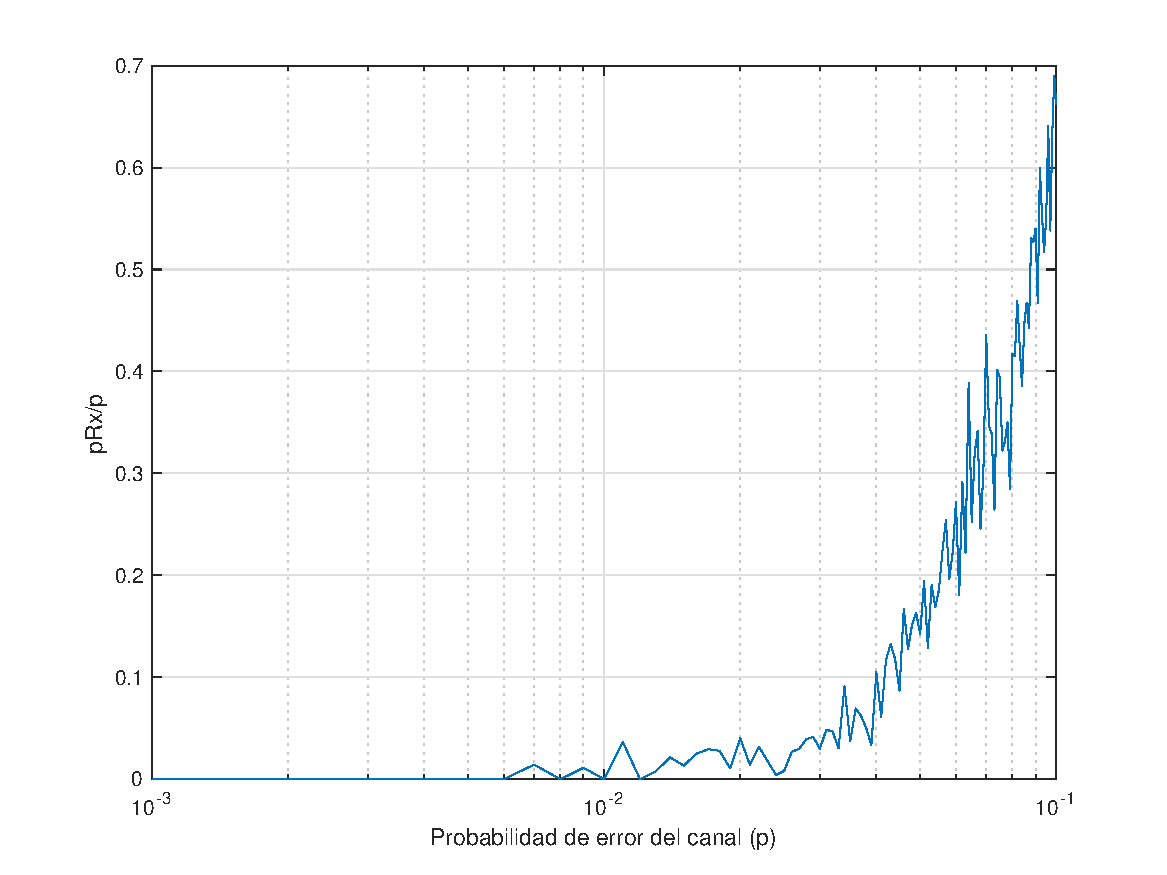
\includegraphics[width=8cm]{./Figuras/Figura1.pdf}

Se define ganancia de codificación como la diferencia entre la relación señal a ruido que se necesita para obtener una determinada probabilidad de error sin utilizar codificación y utilizándola. Con esto en mente, ¿veis algo extraño en la gráfica anterior?

\section{¿Qué entregar?}
\begin{itemize}
	\item Todas las funciones creadas.
\end{itemize}


%\printindex
\end{document}



	
